\documentclass{beamer}
\usepackage{amsmath,amsbsy,amsopn,amstext,amsfonts,amssymb}
\usepackage{isomath}
\usepackage{ulem}
%\linespread{1.6}  % double spaces lines
\usepackage{graphicx}
\usepackage{subfigure}
\usepackage{color}
\usepackage{optidef}  % define optimization problems
\usepackage{multicol}  % multiple columns
\usepackage{listings} % for python code
\usepackage{mathrsfs}

\usepackage{polynom}
\newcommand{\adj}{\mathrm{adj}}
\newcommand{\constrainedmin}[3]{
		\begin{mini*}|s|
		{#2}{#1}{}{}
		\addConstraint{#3}
		\end{mini*}
}

\newcommand{\rwbcomment}[1]{{\color{blue}RWB:#1}}
\newcommand{\defeq}{\stackrel{\triangle}{=}}
\newcommand{\abs}[1]{\left|#1\right|}
\newcommand{\norm}[1]{\left\|#1\right\|}
\newcommand{\iprod}[1]{\left<#1\right>}
\newcommand{\ellbf}{\boldsymbol{\ell}}
\newcommand{\nubf}{\boldsymbol{\nu}}
\newcommand{\mubf}{\boldsymbol{\mu}}
\newcommand{\abf}{\mathbf{a}}
\newcommand{\bbf}{\mathbf{b}}
\newcommand{\cbf}{\mathbf{c}}
\newcommand{\dbf}{\mathbf{d}}
\newcommand{\ebf}{\mathbf{e}}
\newcommand{\fbf}{\mathbf{f}}
\newcommand{\gbf}{\mathbf{g}}
\newcommand{\hbf}{\mathbf{h}}
\newcommand{\ibf}{\mathbf{i}}
\newcommand{\jbf}{\mathbf{j}}
\newcommand{\kbf}{\mathbf{k}}
\newcommand{\lbf}{\mathbf{l}}
\newcommand{\mbf}{\mathbf{m}}
\newcommand{\nbf}{\mathbf{n}}
\newcommand{\obf}{\mathbf{o}}
\newcommand{\pbf}{\mathbf{p}}
\newcommand{\qbf}{\mathbf{q}}
\newcommand{\rbf}{\mathbf{r}}
\newcommand{\sbf}{\mathbf{s}}
\newcommand{\tbf}{\mathbf{t}}
\newcommand{\ubf}{\mathbf{u}}
\newcommand{\vbf}{\mathbf{v}}
\newcommand{\wbf}{\mathbf{w}}
\newcommand{\xbf}{\mathbf{x}}
\newcommand{\ybf}{\mathbf{y}}
\newcommand{\zbf}{\mathbf{z}}
\newcommand{\Jbf}{\mathbf{J}}
\newcommand{\Acal}{\mathcal{A}}
\newcommand{\Bcal}{\mathcal{B}}
\newcommand{\Lcal}{\mathcal{L}}
\newcommand{\Ncal}{\mathcal{N}}
\newcommand{\Rcal}{\mathcal{R}}
\definecolor{darkolivegreen}{rgb}{0.33, 0.42, 0.18}

\makeatletter
\newenvironment<>{proofstart}[1][\proofname]{%
    \par
    \def\insertproofname{#1\@addpunct{.}}%
    \usebeamertemplate{proof begin}#2}
  {\usebeamertemplate{proof end}}
\newenvironment<>{proofcont}{%
  \setbeamertemplate{proof begin}{\begin{block}{}}
    \par
    \usebeamertemplate{proof begin}}
  {\usebeamertemplate{proof end}}
\newenvironment<>{proofend}{%
    \par
    \pushQED{\qed}
    \setbeamertemplate{proof begin}{\begin{block}{}}
    \usebeamertemplate{proof begin}}
  {\popQED\usebeamertemplate{proof end}}
\makeatother

\title{ECEn 671: Mathematics of Signals and Systems}
\author{Randal W. Beard}
\institute{Brigham Young University}
\date{\today}

\begin{document}

%-------------------------------
\begin{frame}
	\titlepage
\end{frame}


%%%%%%%%%%%%%%%%%%%%%%%%%%%%%%%%%%%%%%%%%%%%%%%%%%%%%%%%%%%%%%%%%
\section{Fundamental Subspaces}
\frame{\sectionpage}

%----------------------------------
\begin{frame}\frametitle{Fundamental Subspaces}
	Let $\Acal: \mathcal{H}_1 \to \mathcal{H}_2$ where $\mathcal{H}_1$ and $\mathcal{H}_2$ are Hilbert spaces. \\
	Then $\Acal^\ast:\mathcal{H}_2 \to \mathcal{H}_1$ and we have the following picture:\\
	\begin{center}
		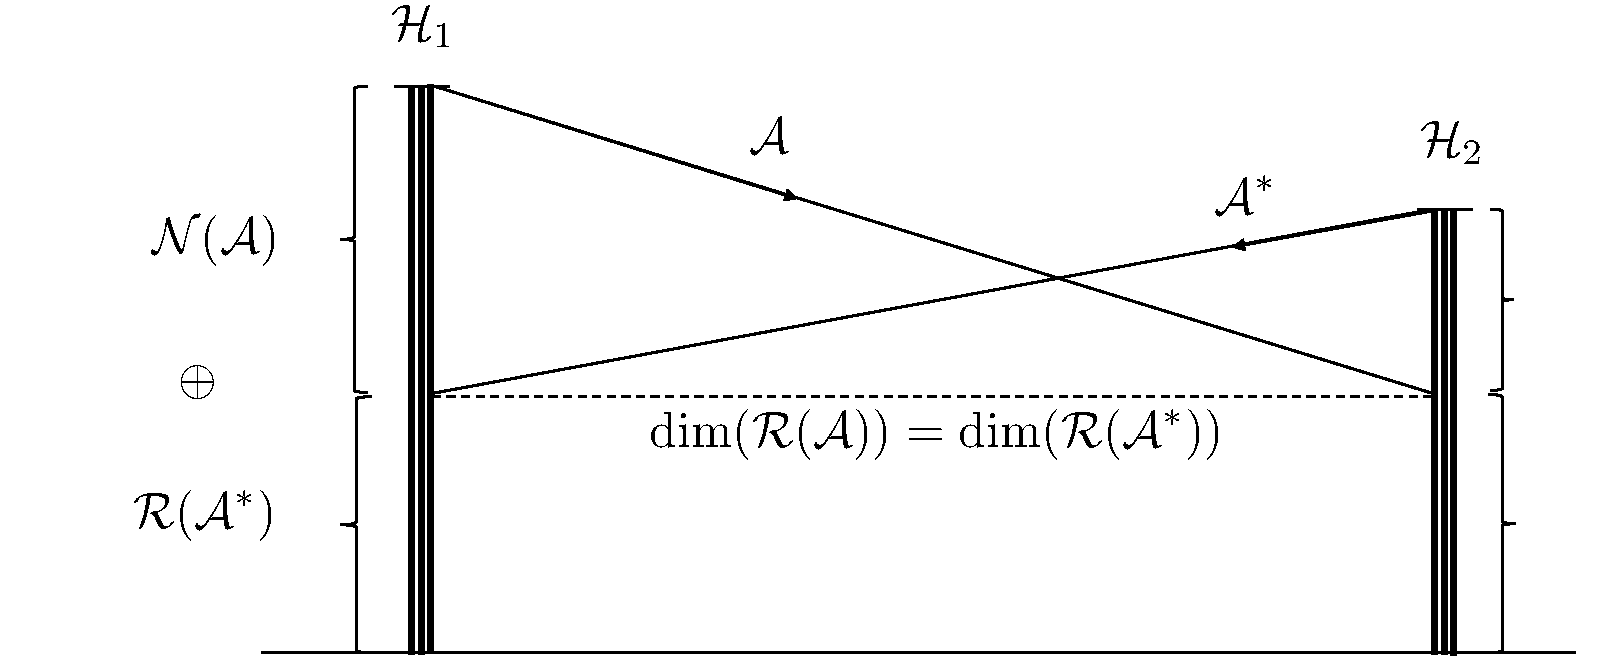
\includegraphics[width=4in]{figures/chap4_fundamental_subspaces}\\
	\end{center}
\end{frame}

%----------------------------------
\begin{frame}\frametitle{Fundamental Subspaces, cont.}
	\begin{lemma}
		\begin{enumerate}
		\item $\mathcal{H}_1 = \mathcal{N}(\Acal) \oplus \mathcal{R}(\Acal^\ast)$
		\item $\mathcal{H}_2 = \mathcal{N}(\Acal^\ast) \oplus \mathcal{R}(\Acal)$
		\item $\dim(\mathcal{H}_1) = \dim(\mathcal{N}(\Acal)) + \dim(\mathcal{R}(\Acal^\ast))$
		\item $\dim(\mathcal{H}_2) = \dim(\mathcal{N}(\Acal^\ast)) + \dim(\mathcal{R}(\Acal))$\\
		\item $\dim(\mathcal{R}(\Acal)) = \dim(\mathcal{R}(\Acal^\ast))$
		\end{enumerate}
	\end{lemma}
	
	Proofs to follow.
	
\end{frame}

%----------------------------------
\begin{frame}\frametitle{Fundamental Subspaces for Matrices}
	For matrices, the picture looks as follows:
	\[ A:\mathbb{C}^n \to \mathbb{C}^m \]
	\[ A^\ast = A^H: \mathbb{C}^m \to \mathbb{C}^n\]
	\begin{center}
		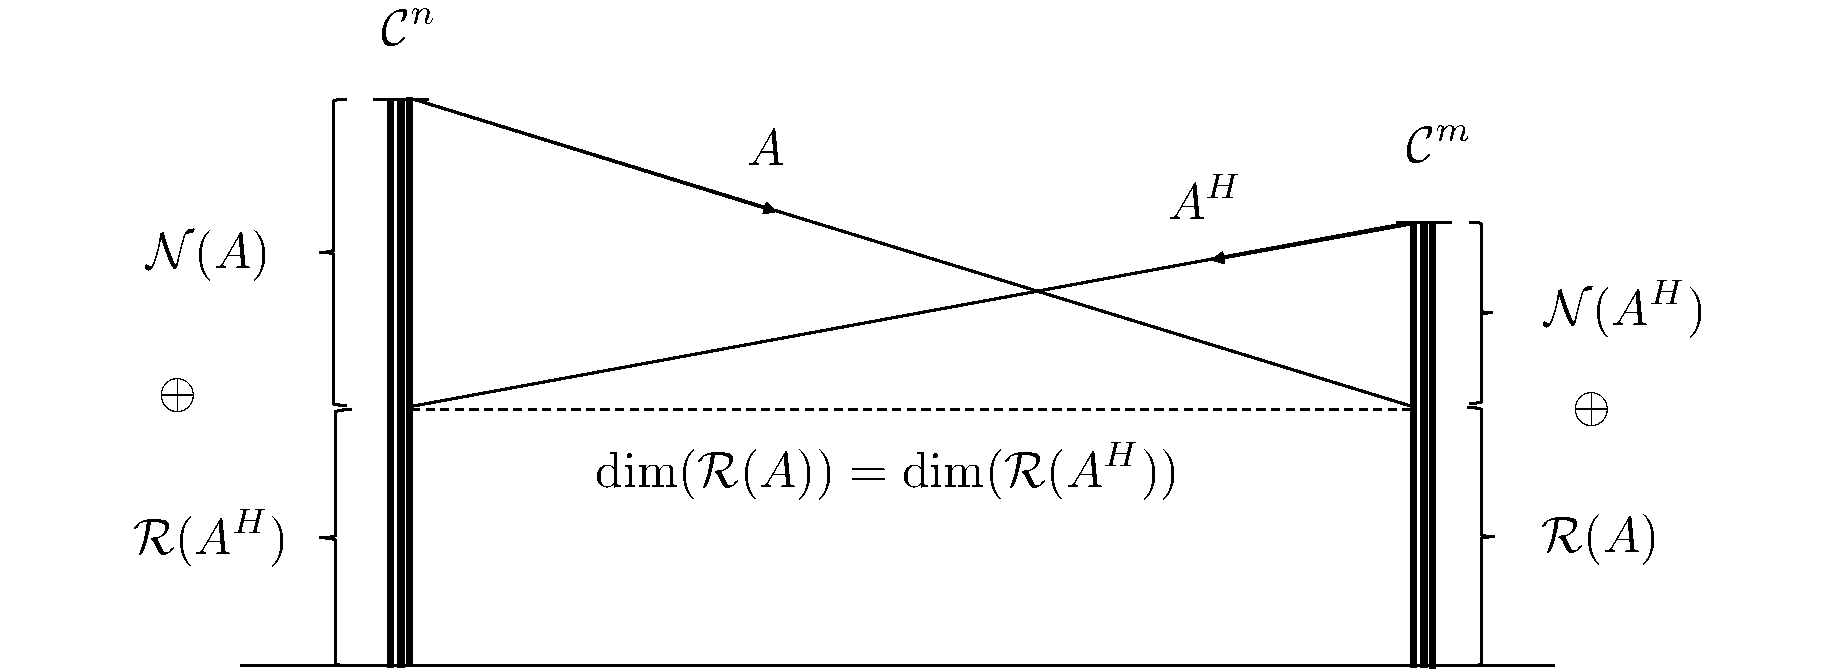
\includegraphics[width=4in]{figures/chap4_fundamental_subspace_matrices}
	\end{center}
	\[\dim(\mathcal{R}(A^H)) = \dim(\mathcal{R}(A))\]
\end{frame}

%----------------------------------
\begin{frame}\frametitle{Fundamental Subspaces, cont}
	\begin{theorem}[Moon Theorem 4.5]	
		Let $\Acal: \mathcal{H}_1 \to \mathcal{H}_2$ be bounded and let $\mathcal{H}_1$ and $\mathcal{H}_2$ be Hilbert spaces and let $\mathcal{R}(\Acal)$ and $\mathcal{R}(\Acal^\ast)$ be closed, then
		\begin{enumerate}
		\item $\left[ \mathcal{R}(\Acal) \right]^{\perp} = \mathcal{N}(\Acal^\ast) $
		\item $\left[ \mathcal{R}(\Acal^\ast) \right]^{\perp} = \mathcal{N}(\Acal) $
		\end{enumerate}	
	\end{theorem}
\end{frame}

%----------------------------------
\begin{frame}\frametitle{Theorem 4.5, Proof}
	\underline{(1):}  To show that $\left[ \mathcal{R}(\Acal) \right]^{\perp} = \mathcal{N}(\Acal^\ast)$ we need to show that $\mathcal{N}(\Acal^{\perp}) \subseteq \left[\mathcal{R}(\Acal)\right]^{\perp}$ and $\left[ \mathcal{R}(\Acal)\right]^{\perp} \subseteq \mathcal{N}(\Acal^\ast)$.
	
	\vfill
	
	\underline{We first show that $\mathcal{N}(\Acal^\ast) \subseteq \left[\mathcal{R}(\Acal)\right]^{\perp}$:}
	
	\vfill
	
	Select any $y \in \mathcal{N}(\Acal^\ast)$ and any $\hat{y} \in \mathcal{R}(\Acal)$.  
	Then $\exists \hat{x} \in \mathcal{H}_1$ such that $\hat{y} = \Acal\hat{x}$.  Therefore
	\begin{align*}
		\iprod{\hat{y}, y } &= \iprod{\Acal\hat{x},y } \\
			&= \iprod{\hat{x}, \Acal^\ast y }\\
			&= \iprod{\hat{x}, 0 } = 0 \\
		\Rightarrow &\quad y \in \left[ \mathcal{R}(\Acal) \right]^{\perp} \\
		\Rightarrow &\quad \mathcal{N}(\Acal^\ast) \subseteq \left[\mathcal{R}(\Acal)\right]^{\perp}
	\end{align*}
\end{frame}

%----------------------------------
\begin{frame}\frametitle{Theorem 4.5, Proof, cont.}

	\underline{We first show that $\left[ \mathcal{R}(\Acal)\right]^{\perp} \subseteq \mathcal{N}(\Acal^\ast)$:}
	
	\vfill
	
	Select any $y \in \left[ \mathcal{R}(\Acal)\right]^{\perp}$.  For every $\hat{x} \in \mathcal{H}_1$ we have $\hat{y} = \Acal\hat{x}\in\Rcal(\Acal)$, and therefore
	\[ \iprod{\hat{y},y }= \iprod{\Acal\hat{x},y } = 0 \]
	By definition of the adjoint, we therefore have that
	\[ \iprod{\hat{x}, \Acal^\ast y } = 0 \]
	Since this is true for every $\hat{x} \in \mathcal{H}_1$ it must be that $\Acal^\ast y = 0$.  Therefore
	\[ y \in \mathcal{N}(\Acal^\ast), \]	
	which implies that
	\[\left[ \mathcal{R}(\Acal)\right]^{\perp} \subseteq \mathcal{N}(\Acal^\ast).\]
	
	\vfill
	
	Item (2) is shown similarly.
\end{frame}

%----------------------------------
\begin{frame}\frametitle{Fundamental Subspaces, cont}
	Theorem 2.10 states that if $\mathcal{H}$ is a Hilbert space and if $\mathbb{V}$ a closed subspace in $\mathcal{H}$ then
	\[ \mathcal{H} = \mathbb{V} \oplus \mathbb{V}^{\perp} \]
	
	\vfill
	
	Therefore Theorem 4.5 implies that
	\begin{align*}
		\mathcal{H}_1 &= \mathcal{R}(\Acal^\ast) \oplus \mathcal{N}(\Acal) \\
		\mathcal{H}_2 &= \mathcal{R}(\Acal) \oplus \mathcal{N}(\Acal^\ast)
	\end{align*}
	
	\vfill
	
	Which also implies that
	\begin{align*}
		\dim(\mathcal{H}_1) &= \dim(\mathcal{R}(\Acal^\ast)) + \dim(\mathcal{N}(\Acal)) \\
		\dim(\mathcal{H}_2) &= \dim(\mathcal{R}(\Acal)) + \dim(\mathcal{N}(\Acal^\ast))
	\end{align*}
\end{frame}

%----------------------------------
\begin{frame}\frametitle{Fundamental Subspaces, cont}
	\begin{columns}
		\begin{column}{0.5\textwidth}
				\begin{lemma}
					\begin{itemize}
						\item $\mathcal{R}(\Acal) = \mathcal{R}(\Acal\Acal^\ast)$
						\item $\mathcal{R}(\Acal^\ast) = \mathcal{R}(\Acal^\ast\Acal)$
					\end{itemize}
				\end{lemma}
		\end{column}
		\begin{column}{0.5\textwidth}
			\begin{center}
				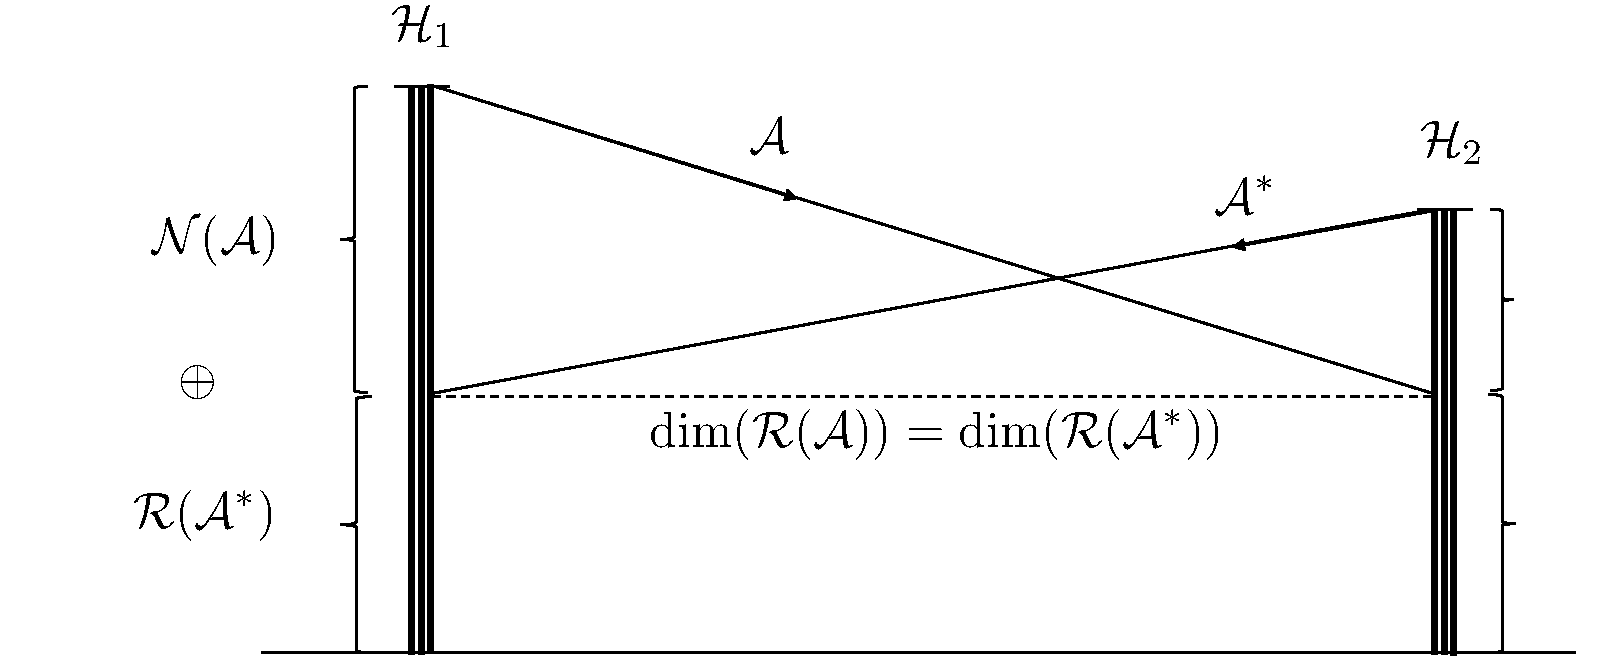
\includegraphics[width=\textwidth]{figures/chap4_fundamental_subspaces}
			\end{center}	
		\end{column}
	\end{columns}

	\begin{proofstart}
		We will prove (1) by showing that:
		\begin{description}
		\item[(a)] 	$\mathcal{R}(\Acal) \subseteq \mathcal{R}(\Acal\Acal^\ast)$
		\item[(b)]  $\mathcal{R}(\Acal\Acal^\ast) \subseteq \mathcal{R}(\Acal)$
		\end{description}
	\end{proofstart}
	
\end{frame}

%----------------------------------
\begin{frame}\frametitle{Fundamental Subspaces, cont}
	\begin{proof}[Proof (cont.)]
		\noindent (a) Let $y \in \mathcal{R}(\Acal) \Rightarrow \exists x \in \mathcal{H}_1 $ such that $ y = \Acal x$

		Since $\mathcal{H}_1 = \mathcal{R}(\Acal^\ast) \oplus \mathcal{N}(\Acal), \quad x  = x_n + x_r$ where
		\[ x_n \in \mathcal{N}(\Acal) \text{ and } x_r \in \mathcal{R}(\Acal^\ast) \]
		\[ \Rightarrow \exists \hat{y} \in \mathcal{H}_2 \text{ such that } x_r = \Acal^\ast\hat{y}\]
		so
		\[ y = \Acal x = \Acal(x_n + x_r) = \Acal\Acal^\ast\hat{y} \]
		\[ \Rightarrow y \in \mathcal{R}(\Acal\Acal^\ast) \]	 
		
		\noindent (b) let $y \in \mathcal{R}(\Acal\Acal^\ast) \Rightarrow \exists \hat{y} \in \mathcal{H}_2 $ such that
		\[ y = \Acal\Acal^\ast\hat{y} \Rightarrow y = \Acal\hat{x} \text{ where } \hat{x} \in \mathcal{H}_1 \]
		\[ \Rightarrow y \in \mathcal{R}(\Acal). \]	
	\end{proof}
	
\end{frame}

%----------------------------------
\begin{frame}\frametitle{Fundamental Subspaces, cont}
	\begin{theorem}
		\[ 
		\dim(\Rcal(\Acal)) = \dim(\Rcal(\Acal^\ast)) 
		\]
	\end{theorem}
	
	\begin{proofstart}
		We need to show that
		\begin{description}
			\item[(a)] $ \dim(\Rcal(\Acal)) \leq \dim(\Rcal(\Acal^\ast)) $
			\item[(b)]\ $ \dim(\Rcal(\Acal^\ast)) \leq \dim(\Rcal(\Acal)) $
		\end{description}
	\end{proofstart}
\end{frame}

%----------------------------------
\begin{frame}\frametitle{Fundamental Subspaces, cont}
	\begin{proofstart}[Proof (cont.)]
		(a) Let $P = \{ p_1, p_2, \ldots \}$ be a Hamel basis for $\mathcal{R}(\Acal)$ so $\dim(\mathcal{R}(\Acal)) = \mathit{cardinality}$ of $P$.
		\[ p_i \in \mathcal{R}(\Acal) \Rightarrow \exists \hat{q}_i \in \mathcal{H}_1 \text{ such that } p_i = \Acal\hat{q}_i \]
		\[ \mathcal{H}_1 = \mathcal{R}(\Acal^\ast) \oplus \mathcal{N}(\Acal) \Rightarrow \hat{q}_i = q_{i,n} + q_i \]
		\[ \text{ where } q_{i,n} \in \mathcal{N}(\Acal) \text{ and } q_i \in \mathcal{R}(\Acal^\ast) \]
		\[ \Rightarrow p_i = \Acal q_i,\] let
		\[ Q = \{ q_1, q_2, \ldots \} \] we will show that $Q$ is linearly independent $\Rightarrow $ any Hamel basis of $\mathcal{R}(A^\ast)$ contains $Q \Rightarrow \dim(\mathcal{R}(A^\ast)) \geq \dim(\mathcal{R}(A))$,


	\end{proofstart}
\end{frame}

%----------------------------------
\begin{frame}\frametitle{Fundamental Subspaces, cont}
	\begin{proof}[Proof (cont.)]
		$P$ is a Hamel basis $\Rightarrow$ all finite subsets of $P$ are linearly independent, i.e.
		\[ \sum_{i \in I} c_ip_i = 0 \iff c_i = 0, i \in I \]
		where $I$ is a finite index set.  But,
		\[ \sum_I c_ip_i = 0 \iff \sum_I c_i\Acal q_i = 0 \iff \Acal(\sum_I c_iq_i) = 0 \]
		but
		$ \sum_I c_i q_i \in \mathcal{R}(\Acal^\ast) \perp \mathcal{N}(\Acal) $\\
		so
		\[ \iff \sum_I c_i q_i = 0 \iff c_i = 0, i \in I \]
		\[ \Rightarrow Q \text{ is linearly independent } \]
		
		(b) Substitute $\Acal$ for $\Acal^\ast$ and $\Acal^\ast$ for $\Acal$ is above argument.

	\end{proof}
	
\end{frame}


%----------------------------------
\begin{frame}\frametitle{Solution of Operator Equations}
	We turn to solutions to the linear operator equation
	\[ \Acal x = y \]
	where $\Acal:\mathcal{H}_1 \to \mathcal{H}_2 $ is bounded, $\mathcal{H}_1$ and $\mathcal{H}_2$ are Hilbert and $\mathcal{R}(\Acal)$ is closed.
	
		\begin{multicols}{2}
			\begin{description}
			\item[Fact 1.]	$\Acal x = y$ has a solution $\iff y \in \mathcal{R}(\Acal) $
			\item[Fact 2.] $\Acal x = y$ has a solution $\iff y \perp \mathcal{N}(\Acal^\ast)$
			\end{description}
 
			\columnbreak

			\begin{center}
				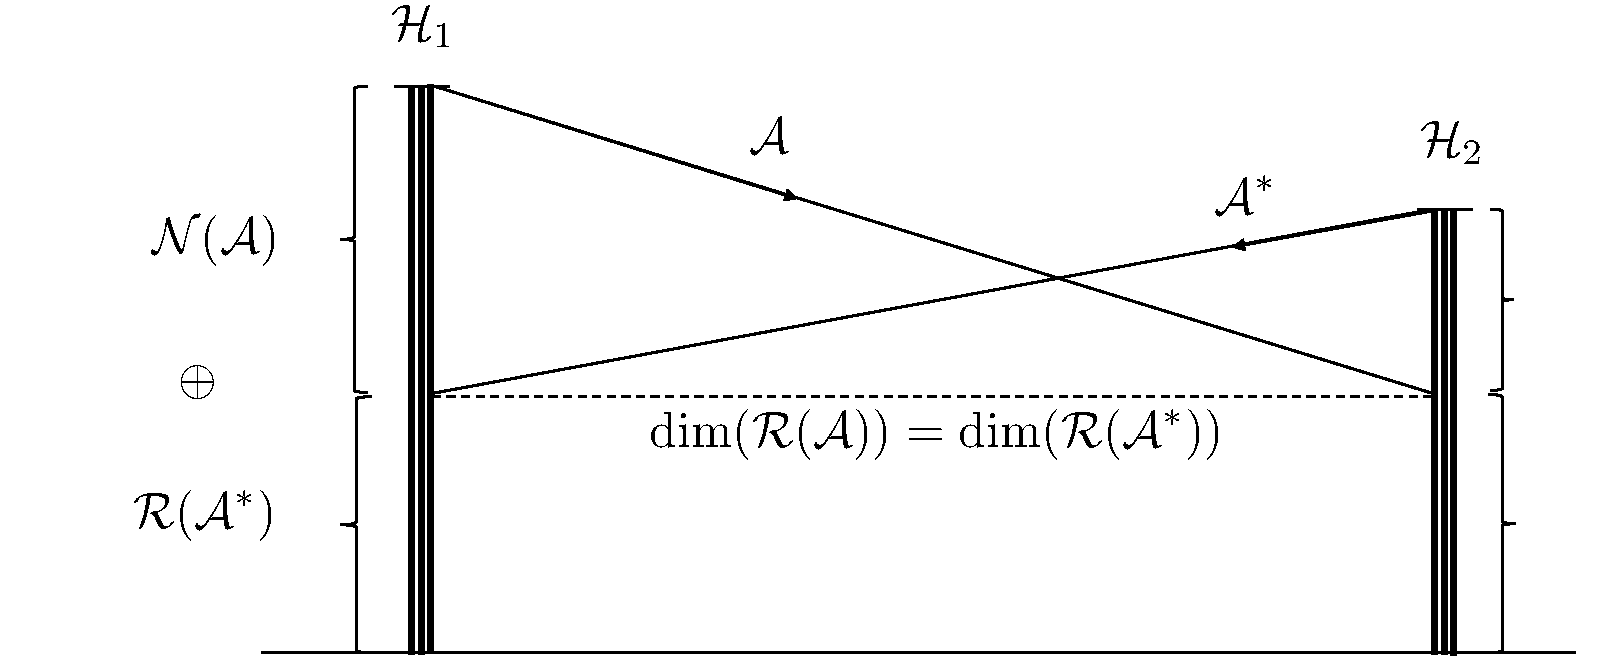
\includegraphics[width=2in]{figures/chap4_fundamental_subspaces}
			\end{center}	
		\end{multicols}

\end{frame}

%----------------------------------
\begin{frame}\frametitle{Solution of Operator Equations}
	\begin{description}
		\item[Fact 3.] If $\Acal x = y$ has a solution then it is unique $\iff \mathcal{N}(\Acal) = \{0\}$
		\item[Fact 4.]  If $\mathcal{N}(\Acal) \neq \{0\}$ and $y \in \mathcal{R}(\Acal)$ then $\Acal x = y$ has an infinite number of solutions.
		\item[Fact 5].  $\Acal^{-1}$ exists $\Rightarrow \mathcal{N}(\Acal) = \{0\}$ (otherwise can't get back to all of $\mathcal{H}$.
	\end{description}
 
	\begin{center}
		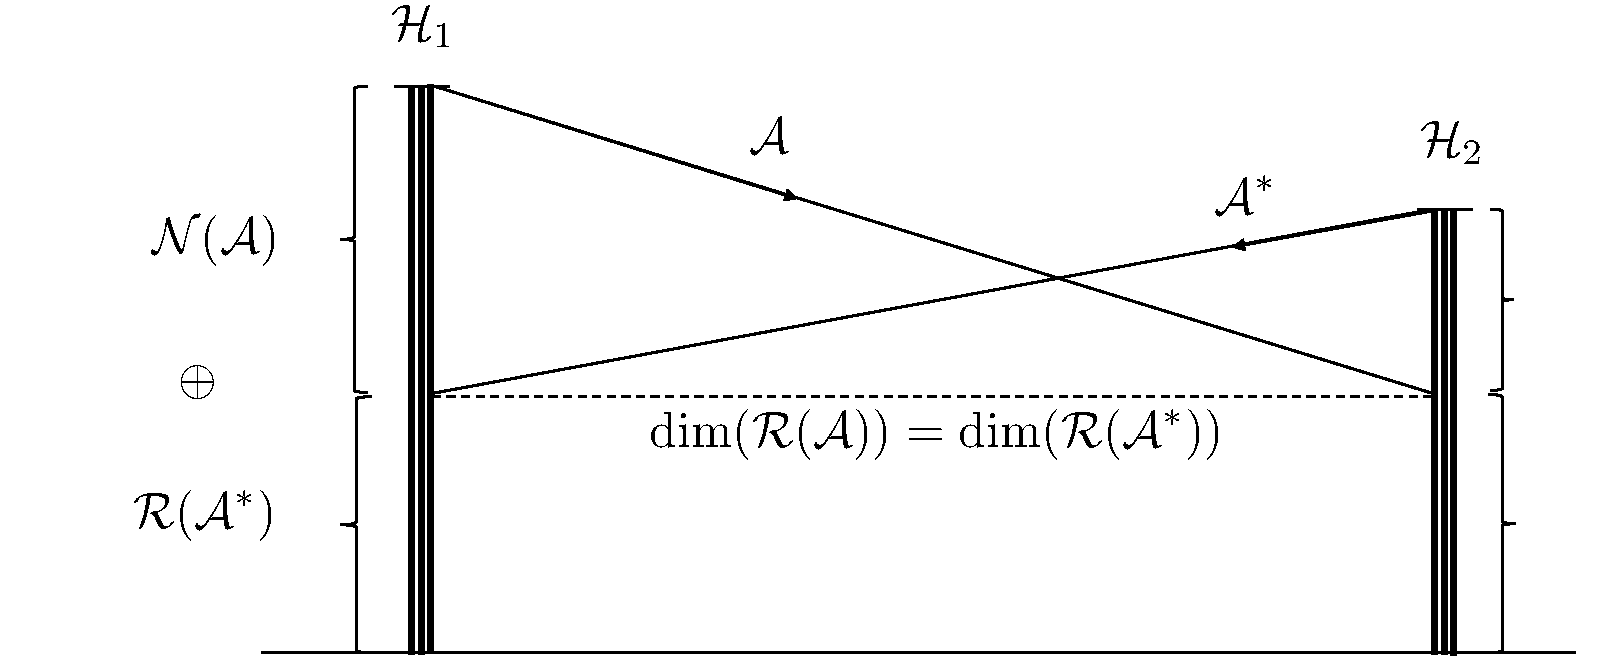
\includegraphics[width=4in]{figures/chap4_fundamental_subspaces}
	\end{center}	
\end{frame}


%----------------------------------
\begin{frame}\frametitle{Matrix Rank}
	\begin{definition}[Row Rank] 
		The \underline{row rank} of $A\in\mathbb{C}^{m\times n}$ is the number of linearly independent rows.
	\end{definition}
	\begin{definition}[Column Rank]
		The \underline{column rank} of $A\in\mathbb{C}^{m\times n}$ is the number of linearly independent columns.
	\end{definition}

	\begin{itemize}
		\item Since $\mathcal{R}(A) = span\{\text{columns of } A\}$ we have that $\dim(\mathcal{R}(A)) = \text{ column rank }$
		\item Since $\mathcal{R}(A^H) = span\{\text{rows of } A\}$ we have that $\dim(\mathcal{R}(A^\ast)) = \text{ row rank } $
		\item Therefore $\dim(\mathcal{R}(A)) = \dim(\mathcal{R}(A^H))$ implies that $\text{ column rank } = \text{ row rank }$
	\end{itemize}
\end{frame}

%----------------------------------
\begin{frame}\frametitle{Matrix Rank}
	\begin{definition}
		The rank of $A$ is the number of linearly independent rows or columns.
	\end{definition}
	
	\begin{lemma}
		\[ rank(A) = rank(A^H) \]
	\end{lemma}

	\begin{definition}
		$A: \mathbb{C}^n\to \mathbb{C}^m $ is full rank if $rank(A) = \min(n,m)$
	\end{definition}
	
\end{frame}

%----------------------------------
\begin{frame}\frametitle{Sylvester's Inequality}
	\begin{lemma}[Sylvester's Inequality]
		Let $A \in \mathbb{C}^{q\times n}$ and $B \in \mathbb{C}^{n \times p}$ then 
		\[
			rank(A) + rank(B) - n \leq rank(AB) \leq \min(rank(A),rank(B)).
		\]
	\end{lemma}
	
	\vfill

	\begin{example}
	Let $x \in \mathbb{R}^m$ and $y \in \mathbb{R}^n$ then
	\[ rank(xy^\top) = 1 \]
	
	\end{example}
\end{frame}


\end{document}